\documentclass[dvipdfmx, 9pt, a4paper]{jsarticle}
\usepackage[margin=15mm]{geometry}
\usepackage{fancyhdr}
\usepackage{multirow}
\usepackage{amsmath,  amssymb}
\usepackage{type1cm}
\usepackage{latexsym}
\usepackage{algorithmic}
\usepackage{algorithm}
\usepackage{ascmac}
\usepackage{braket}
\usepackage{listings,jvlisting}
\usepackage{tcolorbox}
\usepackage[utf8]{inputenc}
\usepackage{color}

\renewcommand{\theequation}{\arabic{section}.\arabic{equation}}
\renewcommand{\thefigure}{\arabic{section}.\arabic{figure}}
\renewcommand{\thetable}{\arabic{section}.\arabic{table}}
\makeatletter
\@addtoreset{equation}{section}
\@addtoreset{figure}{section}
\@addtoreset{table}{section}
\AtBeginDocument{
  \renewcommand*{\thelstlisting}{\arabic{section}.\arabic{lstlisting}}%
  \@addtoreset{lstlisting}{section}
}


\numberwithin{equation}{section}

\DeclareFixedFont{\ttb}{T1}{txtt}{bx}{n}{9}
\DeclareFixedFont{\ttm}{T1}{txtt}{m}{n}{9}
\definecolor{deepblue}{rgb}{0,0,0.5}
\definecolor{deepred}{rgb}{0.6,0,0}
\definecolor{deepgreen}{rgb}{0,0.5,0}

\renewcommand{\baselinestretch}{0.78}
\newcommand{\bm}[1]{{\mbox{\boldmath $#1$}}}
\newcommand{\bnabla}{\bm \nabla}
\newtheorem{Proof}{証明}
\def\qed{\hfill $\Box$}

\newcommand\pythonstyle{\lstset{
language=Python,
basicstyle=\ttm,
morekeywords={self},
keywordstyle=\ttb\color{deepblue},
emph={MyClass,__init__},
emphstyle=\ttb\color{deepred},
stringstyle=\color{deepgreen},
frame=tb,
showstringspaces=false
}}

\lstnewenvironment{python}[1][]
{
\pythonstyle
\lstset{#1}
}
{}

\newcommand\pythonexternal[2][]{{
\pythonstyle
\lstinputlisting[#1]{#2}}}
\newcommand\pythoninline[1]{{\pythonstyle\lstinline!#1!}}

\begin{document}
\begin{center}
{\fontsize{18pt}{1pt}\selectfont ガウス過程とベイズ最適化}\\
\end{center}

\section{ガウス過程}
ガウス過程は教師あり学習に分類される手法であり、多くの場合回帰モデルとして利用される。回帰とは一般的に、入力$\bm x \in V$に対する出力$y \in \mathbb{R}$を関数$f:V \to \mathbb{R}$でモデル化する手法である(ここで$V$は入力の定義域)。ひとたび関数$f$が得られれば、教師データ$\mathcal{D}_n=\{(\bm x_i, y_i)|i=1, ..., n\}$にない入力$\bm x^*$に対しても、出力の予測値$f(\bm x^*)$が得られるようになる。\par
ガウス過程による回帰はベイズ統計とノンパラメトリックモデルの性質を兼ね備えている点で特徴的である。パラメトリックなベイズ線形回帰モデルの場合、関数$f$は$f(\bm x)=\bm w^{\rm T}\bm x$のように、$\bm w$というパラメータを有する。そして$\bm w$の事後分布(例えば$p(\bm w|\mathcal{D}_n)$)を計算することで、関数$f$のバラつきを求める。ここで言う「関数$f$のバラつき」とは、入力$\bm x$が与えられたときの、$f(\bm x)$の確率分布$p(f(\bm x)|\bm x)=p(\bm w^{\rm T}\bm x|\bm x)$というより、関数の集合$\{f(\bm x) = \bm w^{\rm T}\bm x|\bm w \in \mathbb{R}^D\}$に対応する確率分布である。従って$\bm w$の事後分布と$f$の事後分布は実質同じものと考えてよい。\par
パラメトリックなベイズ機械学習では、パラメータの事後分布という観点で議論するが、ノンパラメトリックモデルの場合は、後者の「関数の分布」という観点の方が分かりやすい。ところで解析学によると、関数$f$はベクトルとして表現できた。つまり、全ての$\bm x_i \in V$に対して、対応する関数値を$f_i=f(\bm x_i)$とし、それを順不同に並べたベクトル$(f_1, f_2, ...)^{\rm T}$も関数の一表現として扱う。このとき、関数の分布とは多次元ベクトルの確率分布として見なせる。\par
このように、ガウス過程では主に3つのベクトルを扱う。一つは入力$\bm x \in V$であり、他の回帰モデルと同様である。そして出力$y \in \mathbb{R}$であり、実際に対象の系から得られた値である。本資料ではこれを単に出力や観測値と呼ぶことにする。出力をベクトルとして解釈する場合は、関数のベクトルと同様に、$\bm y=(y_1, y_2, ...)^{\rm T}$とする。ここで、$y_i$は入力$\bm x_i$に対応する観測値である。3つ目のベクトルは前述の通り回帰モデルに関するベクトル$\bm f$である。$\bm f$の成分について、$\bm x_i$に対する関数値$f(\bm x_i)$を単に$f_i$と書くことにする。

\subsection{ガウス過程の基礎}
\begin{tcolorbox}[title=定義1.1ガウス過程]
 関数$f:V \to \mathbb{R}$が、$\bm f \sim \mathcal{N}(\bm\mu, K)$に従うとき、$f$のことをガウス過程と言う。ここで$\bm \mu=(\mu(\bm x_1), \mu(\bm x_2), ...)$であり、関数$\mu:V \to \mathbb{R}$のことを平均関数と言う。また、$K_{ij}=k(\bm x_i, \bm x_j)$であり、関数$k:V \times V \to \mathbb{R}$によって定められる。$f$がこのガウス過程に従うことを$f \sim \mathcal{GP}(\mu, k)$と書き表す。
\end{tcolorbox}\par
上記は確率論における定義であるが、機械学習ではガウス過程に従う回帰モデルのことを単にガウス過程と言う。\par
ガウス過程の例としてパラメトリックなベイズ線形回帰を考えよう。いま、線形回帰モデル$f(\bm x)=\sum_{i=1}^H w_i\phi_i(\bm x)$に対し、$\bm w \sim \mathcal{N}(\bm 0, \lambda^2I)$なる事前分布を考える。ここで$\phi:V \to \mathbb{R}$は基底関数であり、今回は$H$個の基底関数を考えている。従って$\bm w \in \mathbb{R}^H$である。集合$V$を$\{\bm x_1, \bm x_2, ....\}$のように書いたとき、この線形回帰モデルは
\begin{equation}
\begin{bmatrix}
f_1 \\ f_2 \\ ...
\end{bmatrix}=
\begin{bmatrix}
\phi_1(\bm x_1) & \phi_2(\bm x_1) & ... & \phi_H(\bm x_1) \\
\phi_1(\bm x_2) & \phi_2(\bm x_2) & ... & \phi_H(\bm x_2) \\
... & & &
\end{bmatrix}
\begin{bmatrix}
w_1 \\ w_2 \\ ... \\ w_H
\end{bmatrix} \notag
\end{equation}
のように書き表される。よって$\bm f$は$\bm w$を線形写像したもので、かつ$\bm w$はガウス分布に従うため、$\bm f$の事前分布も$\bm f \sim \mathcal{N}(\bm 0, \lambda^2\Phi \Phi^{\rm T})$に従うことが分かる。ここで$\Phi$は計画行列である。従ってこのベイズ線形回帰モデルは、$\lambda^2\Phi\Phi^{\rm T}$と整合する関数$k$によって定められたガウス過程$\mathcal{GP}(\bm 0, k)$と言える。\par
上式のようにベイズ線形回帰では基底関数とパラメータを明示的に考えるが、これは時に計算コスト上問題となる。ベイズ線形回帰のパラメータ数は$H$であったことを思い出そう。$H$とは基底関数の数であり、多いほど表現力の高い回帰モデルとなる。基底関数としてガウス基底関数がよく用いられる(図1(a))。厳密でない表現になるが、図1(b)から想像できるように、ガウス基底関数が"密に配置"されるほど表現力の高い回帰モデルとなりそうである。すると、入力$\bm x$の次元$D$が大きくなるほど、各軸方向に対して密に基底関数を配置する必要が出てくるので(図1(c))、入力次元と共に必要な$H$の数も指数関数的に増加することが想像できる。これは正に一種の次元の呪いであり、計算コスト上問題になる理由である。\par

\begin{figure}[b]
\begin{center}
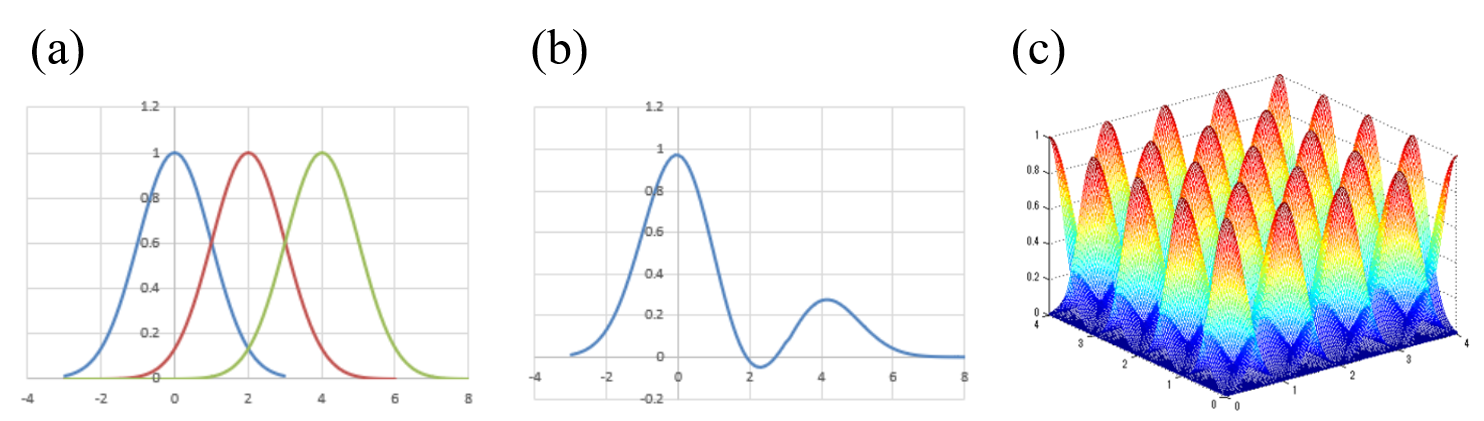
\includegraphics[width=15cm]{fig1.png}
\caption{(a)ガウス基底関数(b)ガウス基底関数を用いた場合の線形回帰モデル(c)2次元入力に対するガウス基底関数}
\end{center}
\end{figure}

一方で、本章で紹介するガウス過程は基底関数の代わりに関数$k$を考える。機械学習の分野では$k$のことをカーネル関数と言う。これまでの議論より、関数の事前分布として知りたいのは$\Phi$ではなく$\lambda^2\Phi\Phi^{\rm T}$であることに気付く。入力$\bm x$が連続値である場合、$V$の元の数は無限であるため、$\Phi \in \mathbb{R}^{\infty \times H}$となる。そのため$\lambda^2\Phi\Phi^{\rm T} \in \mathbb{R}^{\infty \times \infty}$となる。行と列の数が無限になることは置いておくとして(ガウス過程ゆえに解析的な処理が容易なので、計算に困らない)、この行列のサイズが$H$に依存しなくなったことに注目したい。従って、基底関数を定義するのではなく、カーネル関数から直接的に分散共分散行列を定義した場合、$H$の増加による次元の呪いを回避できる。\par
以上がガウス過程の基本的な前提である。このようにガウス過程では基底関数を明示的に考えないので、分散共分散行列も$\lambda^2\Phi\Phi^{\rm T}$ではなく単に$K$と書く。このような行列をカーネル行列と言い、以下のように定義される。
\begin{equation}
K_{i, j}=k(\bm x_i, \bm x_j).
\end{equation}
\subsubsection{ガウス過程のベイズ統計的側面}
先程のベイズ線形回帰モデルは平均関数がゼロのガウス過程という特殊な例であった。平均関数値が常にゼロなのは、暗黙的に存在するパラメータ$\bm w$の期待値をゼロとしたためである。\par
本資料の残りでも平均関数はゼロの定常関数とする。実は教師データ$\mathcal{D}_n=\{(\bm x_i, y_i)|i=1, ..., n\}$に対して観測値$y_i$の平均がゼロとなるように前処理を行えば、平均関数がゼロであっても上手くいくというのが広く知られている。そもそもゼロ以外の平均関数を設定するということは、$\bm w$の期待値を非ゼロに設定することに相当する。これはモデルに対して前提となる知識を有している場合なら上手く働くかもしれないが、あまりそういった機会には出会わない(前提知識を有しているならばパラメトリックな回帰モデルを用いるべきであるため)。従って、ガウス過程の事前分布は以下の通りである。
\begin{equation}
p(\bm f)=\mathcal{N}(\bm 0, K).
\end{equation}\par
次に、回帰モデルに対する観測値の尤度を考える。一般的に回帰モデルと観測値の間に
\begin{equation}
Y=f(\bm x) + \epsilon
\end{equation}
なる関係式を考えることが多い。ここで$\epsilon$は観測誤差に相当する確率変数であり、本資料では$\epsilon \sim \mathcal{N}(0, \sigma^2)$とする。この観測誤差があるゆえに観測値も確率変数として取り扱う。本資料では観測値を$Y$で表し、その実現値を$y$とする。式(1.3)より、尤度は
\begin{equation}
p(\bm Y|\bm f)=\mathcal{N}(\bm f|\sigma^2I)
\end{equation}
となる。ここで$\bm Y=(Y_1, Y_2, ...)$である。これは条件付確率であるため、$\bm f$は実現値であることに注意してほしい(本来なら別の表記にすべきであるが、これが慣習である)。\par
ところで私たちが知りたいのは関数の分布であるが、それは式(1.2)の事前分布ではなく事後分布であり、つまり$p(\bm f|\bm Y_n=\bm y_n)$である。ここで$\bm y_n=(y_1, ..., y_n) \in \mathbb{R}^n$、$\bm Y_n=(Y_1, ..., Y_n) \in \mathbb{R}^n$である。ただし、特に知りたいのは教師データにある入力$X_n=\{\bm x_1, ..., \bm x_n\}$以外の入力$X^*=\{\bm x^*_1, \bm x^*_2, ...\}(X_n^c=X^*)$であろう。そこで関数$\bm f$を$\bm f=(\bm f_n, \bm f^*)^{\rm T}$のように分割して書くことにする。なお$\bm f_n=(f(\bm x_1), ..., f(\bm x_n))^{\rm T} \in \mathbb{R}^n$、$\bm f^*=(f(\bm x^*_1), f(\bm x^*_2), ...)^{\rm T}$である。このとき、$(\bm f_n, \bm f^*)^{\rm T}$の事前分布は
\begin{equation}
p\left(
\begin{bmatrix}
\bm f_n \\ \bm f^*
\end{bmatrix}
\right)=\mathcal{N}\left(
\begin{bmatrix}
\bm 0_n \\ \bm 0^*
\end{bmatrix},
\begin{bmatrix}
K_{ff} & K_{f*} \\
K_{*f} & K_{**} \\
\end{bmatrix}\right) \notag
\end{equation}
のように書き表すことができる。なお、
\begin{equation}
K_{ff}(i, j) = k(\bm x_i, \bm x_j),~~K_{*f}(i, j) = k(\bm x^*_i, \bm x_j),~~K_{f*}(i, j) = k(\bm x_i, \bm x^*_j),~~K_{**}(i, j) = k(\bm x^*_i, \bm x^*_j) \notag
\end{equation}
である。未知の入力に対する事後分布を知りたい場合は、$p(\bm f)$を$\bm f^*$で周辺化すればよい。つまり、
\begin{equation}
p(\bm f^*|\bm y)=\int p(\bm f|\bm y)d\bm f_n=\frac{1}{p(\bm y)}\int p(\bm y|\bm f)p(\bm f)d\bm f \notag
\end{equation}
の計算を行う(最右辺はベイズの定理より導出)。この積分は以下のように求まる。
\begin{equation}
p(\bm f^*|\bm y)=\mathcal{N}(\bm \mu^*, \Sigma^*),~~~\bm \mu^*=K_{*f}(K_{ff}+\sigma^2I)^{-1}\bm y_n,~~~\Sigma=K_{**}-K_{*f}(K_{ff}+\sigma^2I)^{-1}K_{f*}
\end{equation}
$X^*$のうち有限個の入力$X_m=\{\bm x^*_1, ..., \bm x^*_m\}$に対する事後分布のみ知りたい場合は、式(1.5)を更に周辺化すればよい。そこで以下の定理を紹介する。本定理より、カーネル行列の定義を$X_n$と$X_m$に関するものに置き換えれば、式(1.5)と同様であることに気付く。
\begin{itembox}[l]{定理1.1}
 多次元ベクトル$\bm x = (\bm x_1, \bm x_2)^{\rm T}$が以下の分布
\begin{equation}
\begin{bmatrix}
\bm x_1 \\ \bm x_2
\end{bmatrix}=
\mathcal{N}\left(
\begin{bmatrix}
\bm \mu_1 \\ \bm \mu_2
\end{bmatrix}
\begin{bmatrix}
\Sigma_{11} & \Sigma_{12} \\
\Sigma_{21} & \Sigma_{22}
\end{bmatrix}
\right) \notag
\end{equation}
に従うとする。このとき、周辺確率$p(\bm x_1)$は$\mathcal{N}(\bm \mu_1, \Sigma_{11})$である。
\end{itembox}\par

\subsubsection{カーネル関数}
カーネル関数はカーネル行列を決定する重要な関数である。カーネル行列はガウス分布の分散共分散行列となる。分散共分散行列は対称性および半正定値性を有するため、カーネル関数もそれを満たすように設計されていなければならない。つまり、カーネル関数として使えるものは
\begin{equation}
k(\bm x_i, \bm x_j)=k(\bm x_j, \bm x_i), ~~~\sum_{ij}c_ic_jk(\bm x_i, \bm x_j) \geq 0
\end{equation}
を満たす関数に限られる。ここで$c_i(c_j)$は任意の実数である。以下はカーネル関数に関する自明な定理である。
\begin{itembox}[l]{定理1.2}
 関数$k'$及び$k''$が式(1.6)を満たすとき、線形結合$k=ak'+bk''$及び積$k=k'k''$も式(1.6)を満たす。
\end{itembox}\par
カーネル行列が共分散行列であるということは、$k(\bm x_i, \bm x_j)$が$f_i$と$f_j$の共分散となることを意味している。従って対象の問題に対して$f_i$と$f_j$に相関があるならば、$k(\bm x_i, \bm x_j)$も大きな値となるように設計されなければならない。多くの場合において回帰モデルは滑らかな関数とするので、$\bm x_i$と$\bm x_j$の類似度に合わせて大きな値となるカーネル関数を設定する。\par
以下はよく用いられるカーネル関数である。
\begin{itemize}
\item {\bf 線形カーネル}
\begin{equation}
k(\bm x_i, \bm x_j) = \bm x_i^{\rm T}\bm x_j \notag
\end{equation}
\item {\bf 指数カーネル}
\begin{equation}
k(\bm x_i, \bm x_j) = {\rm exp}\left( -\frac{|\bm x_i-\bm x_j|}{\theta} \right) \notag
\end{equation}
ここで$\theta$は正の実数であり、調整可能なパラメータである。$\theta$が小さい程カーネル関数値は小さくなりやすくなる。そのため$\theta$を小さくすることで類似度の判定を厳しくすることができると表現できる。このようなパラメータをスケールパラメータと言う。
\item {\bf RBFカーネル}
\begin{equation}
k(\bm x_i, \bm x_j) = {\rm exp}\left( -\frac{(\bm x_i-\bm x_j)^2}{2l^2} \right) \notag
\end{equation}
ここで$l$はスケールパラメータである。
\item {\bf 周期カーネル}
\begin{equation}
k(\bm x_i, \bm x_j) = {\rm exp}\left(\theta_1{\rm cos}\left( \frac{|\bm x_i-\bm x_j|}{\theta_2} \right)\right) \notag
\end{equation}
ここで$\theta_1, \theta_2$はスケールパラメータである。周期カーネルは$\bm x$の類似度に周期性を持たせている点で特徴的である。
\item {\bf Maternカーネル}
\begin{equation}
k(\bm x_i, \bm x_j)=\frac{2^{1-\nu}}{\Gamma(\nu)}\left( \frac{\sqrt{2\nu}|\bm x_i-\bm x_j|}{\theta} \right)^\nu K\left(\frac{\sqrt{2\nu}|\bm x_i-\bm x_j|}{\theta}\right) \notag
\end{equation}
ここで$\theta$はスケールパラメータ、$\nu$はカーネルの微分特性を調整するパラメータである。また、$K$は第二種の変形ベッセル関数である。$\nu \to \infty$のとき、MaternカーネルはRBFカーネルと一致する。\par
RBFカーネルは解析のしやすさなどの理由ゆえに機械学習の分野でよく採用されていた。一方で、RBFカーネルの無限回微分可能という性質は回帰モデルとして極端な前提であることも指摘されている。そこで、可能な微分回数が調整できるMaternカーネルが提案された次第である。Maternカーネルは$\nu$より大きい自然数の内最小の数だけ微分可能である。$\nu$の値としてよく用いられるのが$3/2$と$5/2$で、それぞれMatern3およびMatern5と呼ばれる。
\begin{equation}
\begin{array}{ll}
(\nu=3/2):&k(\bm x_i, \bm x_j)=\left(1+\frac{\sqrt{3}|\bm x_i-\bm x_j|}{\theta}\right){\rm exp}\left(-\frac{\sqrt{3}|\bm x_i-\bm x_j|}{\theta}\right) \\
(\nu=5/2):&k(\bm x_i, \bm x_j)=\left(1+\frac{\sqrt{5}|\bm x_i-\bm x_j|}{\theta}+\frac{5|\bm x_i-\bm x_j|^2}{3\theta^2}\right){\rm exp}\left(-\frac{\sqrt{5}|\bm x_i-\bm x_j|}{\theta}\right)
\end{array} \notag
\end{equation}
\end{itemize}

\subsubsection{解析結果例(sample.py)}
本資料作成を通して、ガウス過程のためのモジュール「pyGP」を作成した。pyGPは本資料と同じ場所に保存している。以下はsine関数に対する回帰モデル例である。なお、観測誤差としてサンプルデータには標準偏差0.1のガウス分布に従う誤差を加えた。

\begin{figure}[t]
\begin{center}
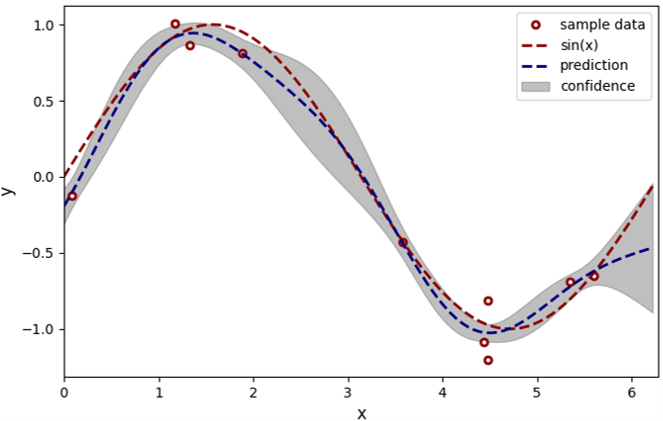
\includegraphics[width=8cm]{fig2.png}
\caption{ガウス過程解析結果例}
\end{center}
\end{figure}

\newpage

\subsection{補助変数法}
本節ではガウス過程の計算コスト対策として提案された補助変数法を紹介する。前述の通り、ガウス過程では行列$K^{nn}+\sigma^2I$の逆行列を求めなければならない。これは$N$行$N$列の行列であるため、ガウスの消去法だと$\mathcal{O}(n^3)$の演算コストを要する。従ってビッグデータの場合問題になってくる。また、密行列ゆえにメモリコストも無視できない。\par
補助変数法は教師データ$\mathcal{D}_n=\{(\bm x_i, y_i)|i=1,...,n\}$の代わりに疑似的なデータ$\{(\bm z_i, u_i)|i=1,...,l\}$を考える。ここで$l<n$である。補助変数法では$\{\bm z_i|i=1,...,l\}$のことを補助変数と言う。\par
疑似データのうち$u_i$は実現値として考えない。それよりも補助変数$\bm z_i$をよしなに決めて、それに対応する確率変数$U_i$を考える。$U_i$は$\bm z_i$における回帰モデルの予測なので、
\begin{equation}
\bm U_l \sim \mathcal{N}(\bm 0, K^{ll})
\end{equation}
を満たす。ここで$\bm U_l=(U_1, ..., U_l)^{\rm T}$、$K^{ll}_{ij}=k(\bm z_i, \bm z_j)$である。\par
補助変数は入力データ$X=\{\bm x_i|i=1,...,n\}$から決められる。最も単純な方法として、$X$からランダムに$l$点選択し、それを補助変数として使うことが考えられる(このやり方をSoD法と言う)。もう少しこだわるならば、クラスタリングの利用が考えられる。例えばK-means法を用いて、$X$を$l$個のカテゴリにクラスタリングし、各分類の代表点(例えば重心)を補助変数として利用する。\par
補助変数法はガウス過程の近似手法であり、近似のさせ方が異なる幾つかの手法の総称である(SoD法はそのうちの一つ)。本資料ではSoRとDTC法、並びにFITC法を紹介する。補助変数法全体において共通している近似は、$\bm U_l$に対する条件付き独立性である。いま、関数$\bm f$を$(\bm f_n, \bm f^*, \bm U_l)^{\rm T}$のように分けて表記する。このとき、
\begin{equation}
p(\bm f_n, \bm f^*)=\int p(\bm f_n, \bm f^*|\bm U_l)p(\bm U_l)d\bm U_l \notag
\end{equation}
が成立する。また、$p(\bm f|\bm U_l=\bm u_l)$と$p(\bm f^*|\bm U_l=\bm u_l)$に関しては式(1.5)より
\begin{equation}
\begin{array}{ll}
p(\bm f|\bm U_l=\bm u_l) & = \mathcal{N}(K_{fu}K_{uu}^{-1}\bm u_l, K_{ff}-Q_{ff}) \\
p(\bm f^*|\bm U_l=\bm u_l) & = \mathcal{N}(K_{*u}K_{uu}^{-1}\bm u_l, K_{**}-Q_{**})
\end{array} \notag
\end{equation}
と厳密に求まる。ここで
\begin{equation}
Q_{ab} \equiv K_{au}K^{-1}_{uu}K_{ub}
\end{equation}
である。一方で、補助変数法は$p(\bm f_n, \bm f^*|\bm U_l)$の計算を効率化するために、近似を施す。特に重要な仮定は$\bm U_l$に対する独立性であり、つまり、$p(\bm f_n, \bm f^*|\bm U_l)=q_n(\bm f_n|\bm U_l)q^*(\bm f^*|\bm U_l)$のように近似する。$q^*$及び$q_n$の定め方は手法によって異なる。

\subsubsection{SoR法}
SoR法は$\bm U_l$と回帰モデルの間に
\begin{equation}
\bm f_n=K_{fu}K^{-1}_{uu}\bm u,~~~\bm f^*=K_{*u}K^{-1}_{uu}\bm u \notag
\end{equation}
なる線形性を仮定する。このとき、$\bm f_n$と$\bm f^*$の同時確率分布は
\begin{equation}
p(\bm f_n, \bm f^*) \simeq \int q_n(\bm f_n|\bm U_l)q^*(\bm f^*|\bm U_l)p(\bm U_l)d\bm U_l=\mathcal{N}
\left(\bm 0,
\begin{bmatrix}
Q_{ff} & Q_{f*} \\
Q_{*f} & Q_{**}
\end{bmatrix}
\right) \notag
\end{equation}
のように求まる。以上より、$\bm f^*$の事後分布は式(1.5)より
\begin{equation}
q(\bm f^*|\bm y)=\mathcal{N}(\bm \mu^*, \bm \Sigma^*),~~~\mu^*=\sigma^{-2}K_{*u}\Sigma K_{uf}\bm y_n,~~~\Sigma^*=K_{*u}\Sigma K_{u*}
\end{equation}
となる(あくまで近似手法なので$p(\bm f^*|\bm y)$ではなく$q(\bm f^*|\bm y)$と書いた)。ここで
\begin{equation}
\Sigma=(\sigma^{-2}K_{uf}K_{fu}+K_{uu})^{-1}
\end{equation}
である。式(1.9)を用いて予測をすればよい。以上より、SoR法は$l$行$l$列の逆行列を計算すれば済むこと、並びに$n$行$n$列の行列を定義しなくてもよいことが分かる。\par
図3(a)に解析結果を示す。平均値は概ねよい結果を示しているものの、分散を過少に評価していることが分かる。
\subsubsection{DTC法}
DTC法はSoR法と同様に線形性を仮定するものの、$p(\bm f^*|\bm U_l)$は厳密な確率分布を用いる。従って、$\bm f_n$と$\bm f^*$の同時確率分布は
\begin{equation}
p(\bm f_n, \bm f^*) \simeq =\mathcal{N}
\left(\bm 0,
\begin{bmatrix}
Q_{ff} & Q_{f*} \\
Q_{*f} & K_{**}
\end{bmatrix}
\right) \notag
\end{equation}
となる。このときの事後分布は
\begin{equation}
q(\bm f^*|\bm y)=\mathcal{N}(\bm \mu^*, \bm \Sigma^*),~~~\mu^*=\sigma^{-2}K_{*u}\Sigma K_{uf}\bm y_n,~~~\Sigma^*=K_{**}-Q_{**}+K_{*u}\Sigma K_{u*}
\end{equation}
となる。平均値はSoR法のときと変わらない一方で、分散共分散行列は$K_{**}-Q_{**}$だけ足されている。証明はしないが$K_{**}-Q_{**}$は正定値行列であるため、DTC法による結果の分散はSoR法のときより大きい。解析結果を図3(b)に示す。

\subsubsection{FITC法}
FITC法はDTC法の同時確率分布に更なる改良を加える。具体的には$Q_{ff}$のうち対角成分のみ$K_{ff}$のものに置き換える。つまり、
\begin{equation}
p(\bm f_n, \bm f^*) \simeq =\mathcal{N}
\left(\bm 0,
\begin{bmatrix}
Q_{ff}-{\rm diag}(Q_{ff}-K_{ff}) & Q_{f*} \\
Q_{*f} & K_{**}
\end{bmatrix}
\right) \notag
\end{equation}
とする。このときの事後分布は
\begin{equation}
q(\bm f^*|\bm y)=\mathcal{N}(\bm \mu^*, \bm \Sigma^*),~~~\mu^*=\sigma^{-2}K_{*u}\Sigma K_{uf}\Lambda^{-1}\bm y_n,~~~\Sigma^*=K_{**}-Q_{**}+K_{*u}\Sigma K_{u*}
\end{equation}
となる。ここで
\begin{equation}
\Lambda={\rm diag}(K_{ff}-Q_{ff}+\sigma^2I)
\end{equation}
である。DTCよりも計算コストは高いが、それでも$n$行$n$列の逆行列の計算を回避している($\Lambda$は対角行列であるため容易に逆行列計算可能)。解析結果を図3(c)に示す。

\begin{figure}[b]
\begin{center}
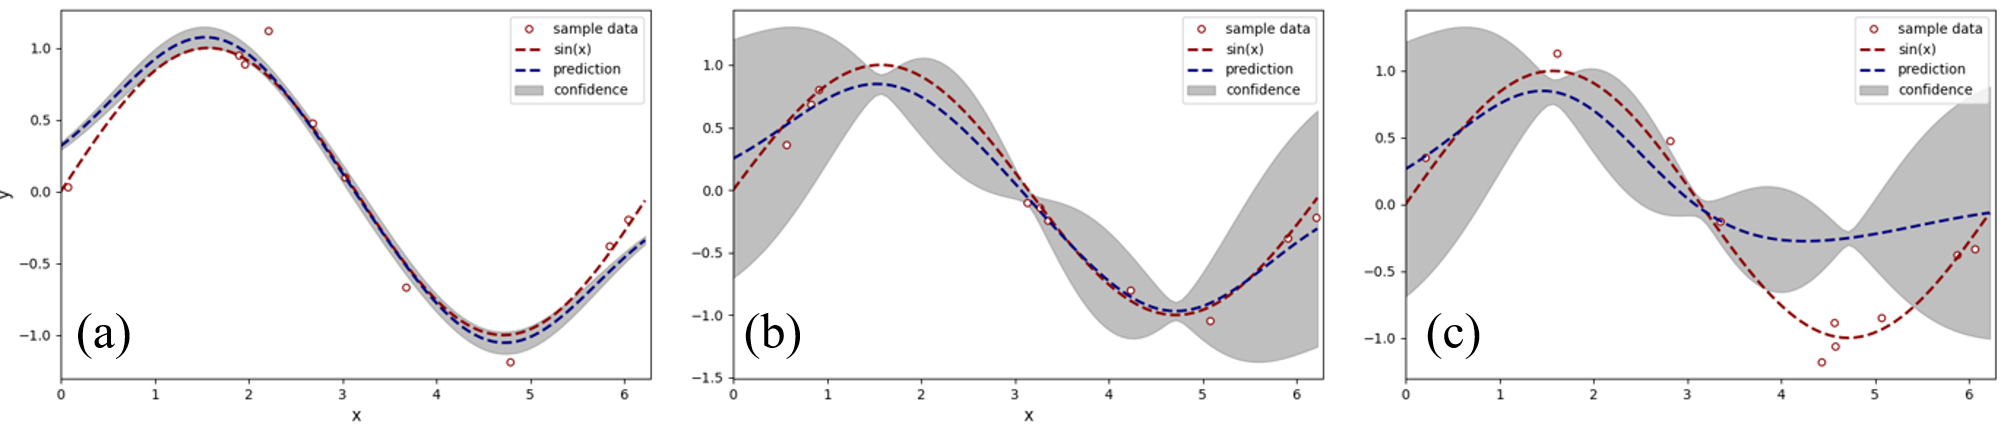
\includegraphics[width=18cm]{fig3.png}
\caption{ガウス過程解析結果例。(a)SoR法(b)DTC法(c)FITC法。}
\end{center}
\end{figure}

\section{ベイズ最適化}
ベイズ最適化とは、数学的に定義された関数の最適解を見つける手法であり、いわゆる最適化手法に分類されるものである。最適化手法には様々な種類があるが、ベイズ最適化は対象の関数にこれといった性質を要求しない(例えば勾配を用いた最適化の場合、関数の微分可能性を要求する)。このような性質をブラックボックス関数に対応可能であると言う。\par
ブラックボックス関数に対応可能な点に着目すれば、ベイズ最適化は進化計算と同類である。しかしながら、ベイズ最適化は対象の関数をベイズ回帰モデル(特にガウス過程回帰)で近似する点で、一般的な進化計算手法と異なる。本資料では、ガウス過程$\bm f \sim \mathcal{N}(\bm 0, K)$でモデル化した場合に限定して議論する。\par
ガウス過程でモデル化するメリットとして、任意の入力$\bm x \in V$における観測値の期待値だけでなく、その自信度合いも定量的に評価できる点にある。後述するように、ベイズ統計は最適化の間逐次的にデータ$(\bm x, y)$を能動的サンプリングして、最終的に最適解が得られるよう設計されている。このプロセスにおいて活用と探索の機構は、他の手法と同様に極めて重要となる。平均関数に注目することは活用に相当し、逆に分散に注目することは探索に相当する。ベイズ最適化は、平均関数$\mu(\bm x)$と分散共分散行列を用いて定義された関数$\alpha:V \to \mathbb{R}$を指針にして次のサンプル点を決め、最適解へ近づいていく。このような関数を獲得関数と言う。\par
ここまでの話を踏まえて、以下にベイズ最適化のアルゴリズムを示す。
\begin{tcolorbox}[title=ベイズ最適化のアルゴリズム]
\begin{enumerate}
\item 初期条件として、$n$個のデータをサンプリングする。つまり、$\mathcal{D}_n=\{(\bm x_i, y_i)|i=1,...,n\}$を得る。なお$n$の値は任意である。
\item $D_n$を用いて式(1.5)等のガウス過程回帰モデルを構築する。
\item 2.のガウス過程回帰モデルに従い、獲得関数が最大となる入力$\bm x_{n+1}={\rm arg~max}_{\bm x \in V}\alpha(\bm x)$を求める。
\item $\bm x_{n+1}$についてサンプリングし、観測値$y_{n+1}$を得る。
\item $\mathcal{D}_{n+1}=\mathcal{D}_n \cup \{(\bm x_{n+1}, y_{n+1})\}$と更新する。
\item 終了条件を満たしていない場合、$n=n+1$とし、2.に戻る。
\item 最終的に得られたデータ$\mathcal{D}_n$のうちの$X_n=\{\bm x_1, ..., \bm x_n\}$に対し、期待関数が最大となる\\$\bm x^*={\rm arg~max}_{\bm x \in X_n}\mu_n(\bm x)$を最適解として出力する。
\end{enumerate}
\end{tcolorbox}\par
獲得関数については様々なモデルが提案されており、その内のいくつかを次節で紹介する。アルゴリズム中3.の$\bm x_{n+1}$を求めるにも、最適値探査が必要となる。これは、獲得関数が微分可能である場合、勾配を用いた最適値探査などで求める。\par
本資料では終了条件について触れない。様々な手法が提案されているが、本資料中の例題はいずれも反復回数の上限を終了条件としている。

\subsection{獲得関数}
\subsubsection{改善確率量獲得関数}
データ$\mathcal{D}_n$が得られた時点における暫定的な最適値$y^*_n$に対し、任意の入力$\bm x \in V$に対する出力$y$がそれよりも最適となる確率を考える。例えば最小値探査の問題である場合、この確率は${\rm Pr}(y < y^*_n)$となる。このあと直ぐに導出するように、この確率は$\bm x$の関数となる。この関数が最大となる$\bm x$は、次のサンプリング点として筋がよい。このような考えに基づく獲得関数を改善確率量獲得関数と言い、以下のように定義する。
\begin{equation}
\alpha(\bm x)={\rm Pr}(y < y^*_n).
\end{equation}\par
暫定的な最適値$y^*_n$は、定義より$y^*_n={\rm min}_i y_i$と書ける。$\mathcal{D}_n$が所与のときのガウス過程回帰モデルの事後分布は式(1.5)で表されるため、任意の$\bm x \in V$における$\alpha(\bm x)$は
\begin{equation}
\alpha(\bm x)=\int_{-\infty}^{y^*_n}\frac{1}{\sqrt{2\pi \sigma^2_n(\bm x)}}{\rm exp}\left(-\frac{(y-\mu_n(\bm x))^2}{2\sigma^2_n(\bm x)}\right)dy \notag
\end{equation}
より求まる。ここで$\mu_n$は$n$個のデータが与えられた段階の平均関数であり、関数$\sigma^2_n(\bm x)$は式(1.5)中$\Sigma$の$\bm x$に対応する対角成分である。つまり、
\begin{equation}
\sigma^2_n(\bm x) = k(\bm x, \bm x) - \bm k_{*f}(\bm x)^{\rm T}(K_{ff}+\sigma^2I)^{-1}\bm k_{f*}(\bm x) \notag
\end{equation}
である。ここで$K_{ff} \in \mathbb{R}^{n \times n}$は$\mathcal{D}_n$に関連するカーネル行列であり、また
\begin{equation}
\begin{array}{ll}
\bm k_{*f}(\bm x) & = (k(\bm x, \bm x_1), ..., k(\bm x, \bm x_n))^{\rm T} \\
\bm k_{f*}(\bm x) & = (k(\bm x_1, \bm x), ..., k(\bm x_n, \bm x))^{\rm T} \\
\end{array}
\end{equation}
である。標準正規分布の累積分布関数$\Phi:\mathbb{R} \to \mathbb{R}$を用いることで、
\begin{equation}
\alpha(\bm x)=\Phi\left( \frac{y^*_n-\mu_n(\bm x)}{\sigma_n(\bm x)} \right)
\end{equation}
を得る。\par
前章で紹介したベイズ最適化のアルゴリズムより、次のサンプル点$\bm x_{n+1}$は式(1.2)を最大とする$\bm x$を選べばよい。改善確率量獲得関数は$\bm x$に関して微分可能であるため、$\bm x_{n+1}$の探査に勾配法を用いることができる。導出過程は省略するが、勾配${\bnabla}\alpha \in \mathbb{R}^D$($D$は$V$の次元数)の第$i$成分$\partial_i\alpha \in \mathbb{R}$は
\begin{equation}
\partial_i\alpha(\bm x)=\phi\left( \frac{y^*_n-\mu_n(\bm x)}{\sigma_n(\bm x)} \right)
\left(\frac{-\partial_i\mu_n(\bm x)\sigma_n(\bm x)+\mu_n(\bm x)\partial_i\sigma_n(\bm x)}{\sigma^2_n(\bm x)}
\right)
\end{equation}
より求まる。ここで関数$\phi:\mathbb{R} \to \mathbb{R}$は標準正規分布関数である。式中に平均関数$\mu_n(\bm x)$と$\sigma_n(\bm x)$の勾配も計算する必要があるが、ガウス過程回帰が$\mathcal{N}(\bm 0, K)$で考えられている場合、それぞれ
\begin{equation}
\begin{array}{ll}
\partial_i\mu_n(\bm x)&=\left(\partial_i\bm k_{*f}(\bm x)\right)^{\rm T}\left(K_n+\sigma^2I\right)^{-1}\bm y_n \\
\partial_i\sigma_n(\bm x)&=\frac{1}{2\sigma_n(\bm x)}\left(\partial_ik(\bm x, \bm x) - \partial_i\bm k_{*f}(\bm x)^{\rm T}\left(K_n+\sigma^2I\right)^{-1}\bm k_{f*}(\bm x) - \bm k_{*f}(\bm x)^{\rm T}\left(K_n+\sigma^2I\right)^{-1}\partial_i\bm k_{f*}(\bm x)\right)
\end{array}
\end{equation}
となる。\par
以上より、改善確率獲得関数を用いた場合のベイズ最適化が導出できた。改善確率獲得関数は最も基本的な関数の一つであり、比較的高速に計算できることが分かっている(データ数$n$に対して$\mathcal{O}(n^2)$。ただしカーネル行列の逆行列計算は除く)。一方で$y^*_n$以下となる確率に注目することは、活用に重きを置きすぎているという指摘もあり、実際に最適化が上手くいかない問題も多い。また、観測誤差が大きい場合も不得意としていることが知られている。

\subsubsection{期待改善獲得関数}
本項で紹介する期待改善獲得関数は、経験的に改善確率獲得関数よりも上手く最適化できることが知られている。期待改善獲得関数は$\alpha(\bm x)=\mathbb{E}({\rm max}(0, y^*_n-y))$のように定義されている。$y^*_n$に着目する点は改善確率獲得関数と同様だが、期待改善獲得関数は確率ではなく差分で定義する。\par
期待改善獲得関数は解析的に求めることができ、
\begin{equation}
\alpha(\bm x)=(y^*_n-\mu_n(\bm x))\Phi\left(\frac{y^*_n-\mu_n(\bm x)}{\sigma_n(\bm x)}\right)+\sigma_n(\bm x)\phi\left(\frac{y^*_n-\mu_n(\bm x)}{\sigma_n(\bm x)}\right)
\end{equation}
である。また、この勾配の第$i$成分は以下の通りである。
\begin{equation}
\partial_i\alpha(\bm x)=-\partial_i\mu_n(\bm x)\Phi\left(\frac{y^*_n-\mu_n(\bm x)}{\sigma_n(\bm x)}\right)+\partial_i\sigma_n(\bm x)\phi\left(\frac{y^*_n-\mu_n(\bm x)}{\sigma_n(\bm x)}\right)
\end{equation}

\subsubsection{信頼下限獲得関数}
信頼下限獲得関数は直感的に分かりやすく理論的な考察も容易であるため、多くの書籍で紹介されている。一方で改善確率獲得関数とは逆に探索圧力が強すぎると言われており、実用上の利用頻度は低い。\par
信頼下限獲得関数は
\begin{equation}
\alpha(\bm x)=-\mu_n(\bm x)+\sqrt{\beta_n}\sigma_n(\bm x)
\end{equation}
のように定義されている。ここで$\beta_n$はハイパーパラメータである。信頼下限獲得関数を最大化する方向に新しい点を探索することで、平均関数値が低くてかつ分散が大きい点をサンプリングするようになる。\par
$\beta_n$の決め方は任意であるが、$\beta_n=({\rm log}n)/n$とすることが多い。ここで$n$は既にサンプリングされたデータの数である。こうすることで、サンプリングされるにつれ活用の圧力を高めることができる。なお、信頼下限獲得関数は探索圧力が強いと指摘している書籍では、$\beta_n=c{\rm log}n$としていた。ここで$c$は実数である。この場合、$\beta_n$は$n$と共に増加していくため、$\beta_n=({\rm log}n)/n$のときと期待する意味合いが真逆である。$c{\rm log}n$の場合に探索圧力が強いのは納得できる。一方で$({\rm log}n)/n$のときも探索圧力が強いと言えるのかについて私は知らない。\par
信頼下限獲得関数の微分は以下の通りである。
\begin{equation}
\partial_i\alpha(\bm x)=-\partial_i\mu_n(\bm x)+\sqrt{\beta_n}\partial_i\sigma_n(\bm x)
\end{equation}

\subsection{制約付きベイズ最適化}
本節では制約付きのベイズ最適化を考える。制約付き最適化の問題設定は様々だが、本資料では
\begin{equation}
{\rm min}f(\bm x),~~~{\rm s.t.}~~c_i(\bm x) \leq 0~(i=1,...,m)
\end{equation}
に統一する。$c(\bm x) \geq 0$の制約を扱いたい場合は$c(\bm x)$の符号を逆転すればよい。また、等式制約は$c(\bm x) \leq 0$かつ$c(\bm x) \geq 0$と考える。そのため、上式のみを考えても一般性を欠くことはない。なお、等式制約について$c(\bm x) \leq 0$かつ$c(\bm x) \geq 0$というのは時に厳しすぎるため、代わりに$c(\bm x) \leq \delta$かつ$c(\bm x) \geq \delta$($\delta \neq 0$)を考えることもある。\par
ブラックボックス関数を扱うベイズ最適化では、関数$c$もブラックボックス関数であることが多い。この場合、ハードな制約を最適値探査時に課すことは難しい。そのため、制約を満足しない解もサンプリングするような手法(ソフトな制約)がベイズ最適化では好まれる。\par
本節で紹介する制約付き最適化の最も特徴的な点は、ブラックボックスな制約関数$c_i$に対してもガウス過程を適用することである。つまり、
\begin{equation}
c_i \sim \mathcal{GP}(0, k_i) \notag
\end{equation}
なる関係を考える。ここで$k_i$は制約関数$c_i$のためのカーネル関数である。$c_i$に対応する観測値を$z^i$とし、観測誤差の分散値を$\sigma'^2$とする。このとき、$z^i$の確率分布は$z^i \sim \mathcal{N}(c_i(\bm x), \sigma'^2I)$に従う。\par
入力点$\bm x_i$に対し、観測値として$y_i$だけでなく$\{z_i^1, ..., z_i^m\}$も得られる。従って教師データは$\mathcal{D}_n=\{(\bm x_i, ..., y_i, z_i^1, ..., z_i^m)|i=1,...,n\}$のように書き表される。

\subsubsection{制約付き期待改善獲得関数}
本項では制約付き獲得関数の例として制約付き期待改善獲得関数を紹介する。\par
まず2.1.2項と比べ、$y_n^*$の選び方が異なる。制約付き期待改善獲得関数においてその選び方は複数あり、Gardnerらは
\begin{equation}
y_n^*={\rm min}\{y_i, | z^j_i \leq 0,~~i=1, ..., n~~~j=1, ..., m\}
\end{equation}
なる選び方、つまり制約を満たすデータの内最小となるものを選ぶ方法を提案している。\par
次に、獲得関数を
\begin{equation}
\alpha(\bm x)=\mathbb{E}\{\Delta(\bm x){\rm max}(0, y^*_n-y_i)\}
\end{equation}
のように定義する。ここで$\Delta(\bm x)$は$\bm x$において全制約を満たす確率である。$c_j(\bm x)$に対応する観測値$z^j$が制約を満たす確率は
\begin{equation}
\int_{-\infty}^0p(z^j|\mathcal{D}_n)=\Phi\left(-\frac{\mu^j_n(\bm x)}{\sqrt{(\sigma^j_n(\bm x))^2+\sigma'^2}}\right) \notag
\end{equation}
となる。ここで$\mu^j_n(\bm x)$はガウス過程$c_j(\bm x)$の平均関数値、$\sigma^j_n(\bm x)$は標準偏差値である。一般的に各制約のガウス過程は独立に従うと仮定されるので、$\Delta(\bm x)$は上式を全制約に対して積を取ったもの、つまり
\begin{equation}
\Delta(\bm x)=\prod_{j=1}^m\Phi\left(-\frac{\mu^j_n(\bm x)}{\sqrt{(\sigma^j_n(\bm x))^2+\sigma'^2}}\right)
\end{equation}
となる。\par
以上より制約付き期待改善獲得関数を定義できた。あとはベイズ最適化のアルゴリズムに従って計算を進めればよい。


\end{document}














